\section{Simulation}

We need to simulate a data set to train, tune and selecting an algorithm for stock picking. As described in section \ref{sec:model} the returns on the stocks are drawn from a distribution (here assumed to be normal):

\begin{equation}
    \rr^{(t)} \sim N(\mu^{(t)}, \Omega^{(t)})
\end{equation}

\subsection{Sampling of expected returns}

Investigating the distribution of means, we find it is reasonable to assume the expected return for an individual stocks follows a normal distribution:

\begin{equation}
    \mu^{(t)}_{i} \sim N(\xi, \sigma_{r})
\end{equation}

To estimate the parameters $\xi$, $\sigma_r$ we perform a log-likelihood estimation which yields the following values: $\xi=0.000461$ and $\sigma_r = 0.00123$. Figure \ref{fig:distmeans} plots the fitted distribution vs. the empirical distribution, and even though the fourth moment of the distribution seems not to exactly follow the normal distribution, the normal distribution appears to be a good approximation of the data generating process of $\mu_i^{(t)}$.

\begin{figure}[ht]
\centering
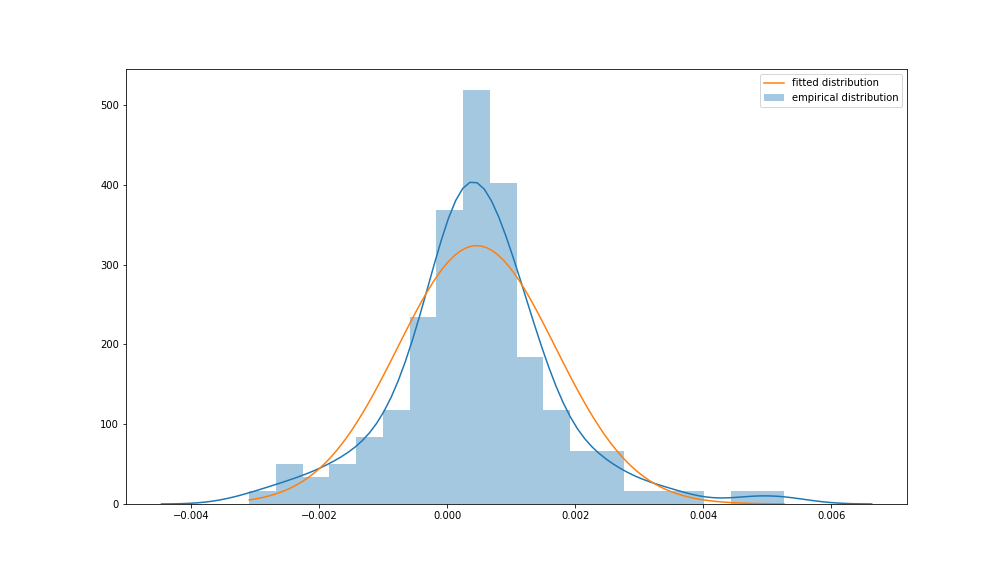
\includegraphics[scale=0.3]{figures/distribution_means.png}
\caption{Distribution of individual means $\mu_i^{(t)}$}
\label{fig:distmeans}
\end{figure}


\subsection{Sampling of covariance matrix}

Sampling the covariance matrix is more involved than sampling $\mu$. I go the following way about in in this paper: Realize that a transformation from a covariance matrix to a correlation matrix is possible:

\begin{equation}
    \text{corr}_{x, y} = \frac{\sigma_{x,y}^{2}}{\sigma_x \cdot \sigma_y}
\end{equation}

Therefore we first need to sample a correlation matrix, then a vector of variances, then transform the correlation matrix to the covariance matrix $\Omega^{(t)}$.

\subsubsection{Sampling of correlation matrix}

Sampling a correlation matrix is not as straightforward as sampling the individual stock returns, $\mu_i^{(t)}$. This is due to the fact, the correlation matrix should adhere to multiple criteria:

\begin{enumerate}
    \item A correlation matrix is a positive definite matrix.
    \item The individual values (apart from the diagonal) of the correlation matrix should follow a normal distribution $\rho_{i}^{(t)} \sim N(\kappa, \sigma_\rho)$.
\end{enumerate}

In this paper to accomplish the desired I use the following sampling scheme:

\begin{enumerate}
    \item Initialize an empty matrix $M$ of size $k \times k$.
    \item sample individual observations $\rho_{i,j}=\rho_{j,i}$ from a fitted normal distribtuion.
    \item Replace the diagonal of $M$ with 1.
    \item Save the matrix $M$ if all eigenvalues are positive, i.e. $M$ is positive definite.
\end{enumerate}

Figure \ref{fig:distcorrs} shows the fitted distribution plotted against the empirical distribution with regards to the individual $\rho_{i,j}^{(t)}$ not considering the diagonal. Again log-likelihood estimation is used to estimate the parameters: $\kappa=0.313, \sigma_\rho=0.188$. Again we see that, the actual distribution does not perfectly follow a normal distribution, but passes for a good approximation. It should be noted that when sampling from this distribution, the distribution is truncated at $(-1, 1)$.

\begin{figure}[ht]
\centering
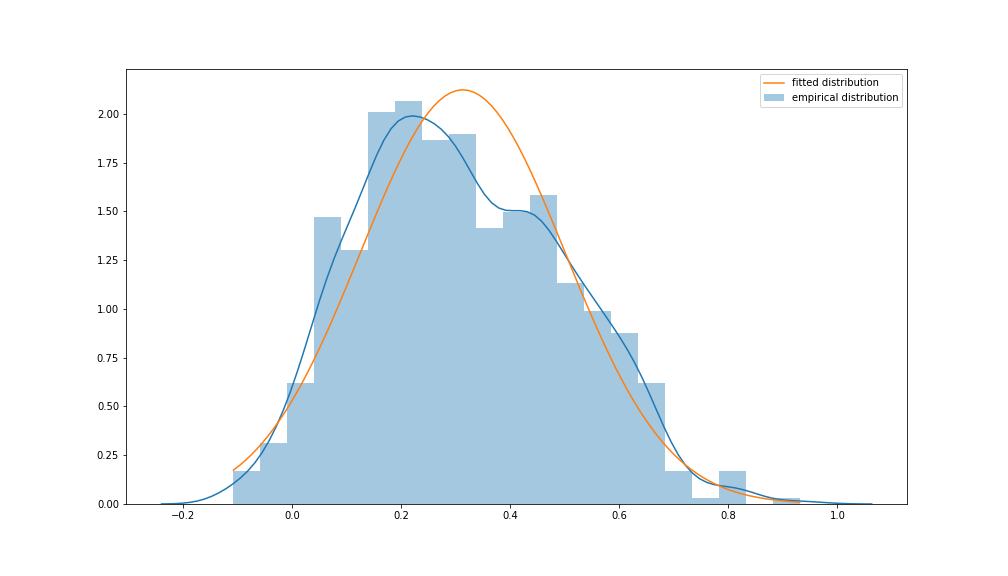
\includegraphics[scale=0.3]{figures/correlation_distribution.png}
\caption{Distribution of individual correlates $\rho_{i,j}^{(t)}$}
\label{fig:distcorrs}
\end{figure}

\subsubsection{Sampling of variances}

The variances does not follow a normal distribution, this is obvious, since the variance by definition is a positive measure. I model the variances to be exponentially distributed: $\sigma^2_{i} \sim expon(\lambda)$. Using log-likelihood estimation we find the $\lambda=0.000346$. Figure \ref{fig:distvars} displays the fitted distribution against the empirical distribution. I conclude that the exponential distribution is a reasonable approximation of the true distribution.

\begin{figure}[ht]
\centering
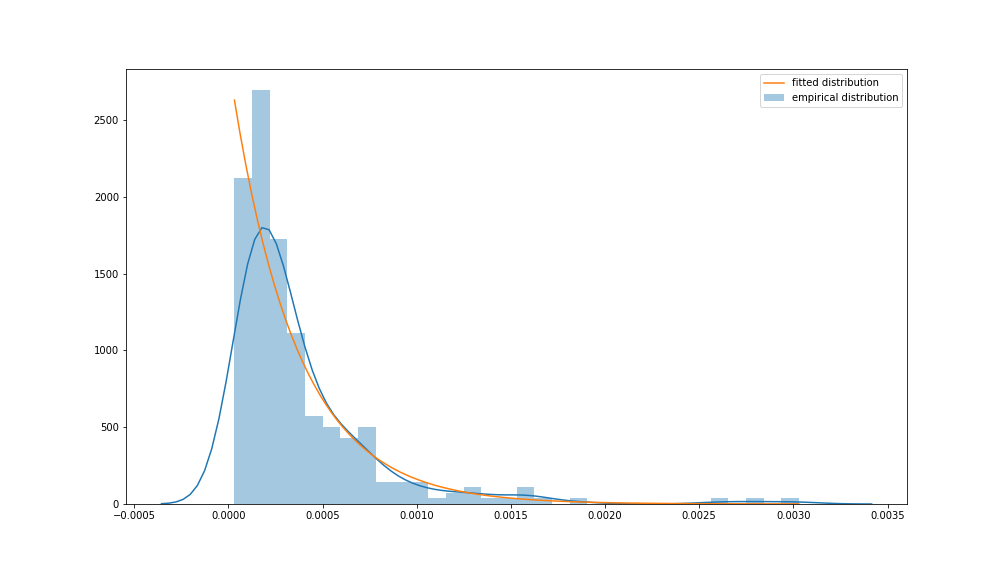
\includegraphics[scale=0.3]{figures/distribution_variances.png}
\caption{Distribution of individual variances}
\label{fig:distvars}
\end{figure}


\subsubsection{The simulated covariance distribution vs. the empirical distribution}

Using the scheme described above, I simulate a set of covariance matrices. Figure \ref{fig:distcovars} displays the simulated distribution of individual covariances vs. the empirical distribution of individual covariances. From the figure, we see that the simulated distribution, seems slightly biased towards 0. However I conclude that for the purpose of this paper the simulation passes as a good approximation.

\begin{figure}[ht]
\centering
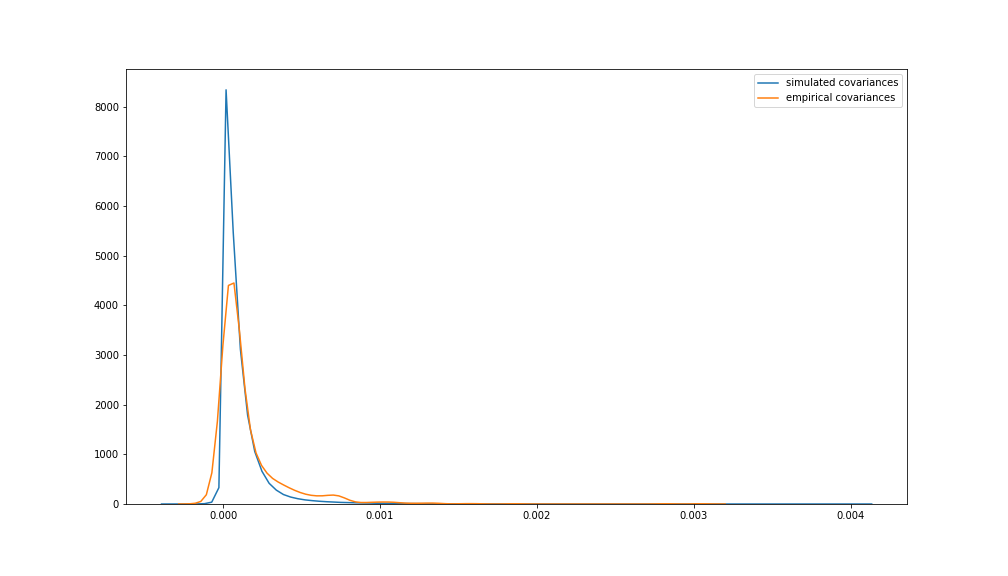
\includegraphics[scale=0.3]{figures/dist_simulated_covariances.png}
\caption{Distribution of individual covariances}
\label{fig:distcovars}
\end{figure}

\subsubsection{The simulated data set}

Now having simulated covariance matrices, and returns, we can simulate an entire data set, that corresponds to our model. We simulate a data set of $11$ columns and $2.000.0000$ rows, which is more than necessary for the further investigation in this paper. We set the parameter $p=0.047$, so we have just slightly less then $10.000$ structural breaks in the simulated data set. Since we have the underlying $\mu^{(t)}$ and $\Omega^{(t)}$ in each period, we can calculate the Sharpe ratios for each of the simulated stocks throughout the period assuming the risk free asset having a return of $\bar{r}=2 \%$ annually.

Summing it all up: A dataset is now constructed based on a structural model. The data set consists of not only the simulated returns, but also the Sharpe ratios of the individual stocks, which in the real data set are latent variables. The simulated data set allows for training, tuning and selecting between algorithms.

